
\begin{name}
	{\tenchude}
	{TOÁN 10}
	{LỚP TOÁN THẦY PHÁT}
	{Thời gian: 30 phút - Không kể thời gian phát đề}
\end{name}
\setcounter{page}{1}
\TN
\Opensolutionfile{ans}[ans/ansBONPA-0D1-OnChuong-De1]
\begin{ex}%[0D1N1-1]
Phát biểu nào sau đây là mệnh đề?
\choice
{Thầy Phát quá 30 tuổi phải không?}
{Bạn có yêu môn Toán không?}
{Cấm học sinh sử dụng điện thoại trong kiểm tra}
{\True Câu C là đáp án đúng của câu hỏi này}
\loigiai{
\lq\lq Câu C là đáp án đúng của câu hỏi này\rq\rq\, là một mệnh đề vì đây là một câu khẳng định sai.
}
\end{ex}

\begin{ex}%[0D1N1-2]
Cho mệnh đề chứa biến $P(x):"3x+5\le x^2"$ với $x$ là số thực. Mệnh đề nào sau đây là đúng?
\choice[2]
{$P(3)$}
{$P(4)$}
{$P(1)$}
{\True $P(5)$}
\loigiai{
\noindent
$P(3)$: "$3\cdot3+5\le 3^2$" $\Leftrightarrow$ "$14\le 9$" là mệnh đề sai.\\
$P(4)$: "$3\cdot4+5\le 4^2$" $\Leftrightarrow$ "$17\le 16$" là mệnh đề sai.\\
$P(1)$: "$3\cdot1+5\le 1^2$" $\Leftrightarrow$ "$8\le 1$ là mệnh đề sai.\\
$P(5)$: "$3\cdot5+5\le 5^2$"$\Leftrightarrow$ "$20\le 25$" là mệnh đề đúng.
}
\end{ex}

\begin{ex}%[0-GHK1-2022, THPT Quốc Học Quy Nhơn - Quy Nhơn, 2021-2022]%[Thành Đức Trung]%[0D1N1-5]
Mệnh đề phủ định của mệnh đề \lq\lq$\forall x \in \mathbb{R}, x^{2}+x+2020>0$\rq\rq\ là
\choice
{\lq\lq$\forall x \in \mathbb{R}, x^{2}+x+2020 \leq 0$\rq\rq}
{\True \lq\lq$\exists x \in \mathbb{R}, x^{2}+x+2020 \leq 0 $\rq\rq}
{\lq\lq$\forall x \in \mathbb{R}, x^{2}+x+2020<0$\rq\rq}
{\lq\lq$\exists x \in \mathbb{R}, x^{2}+x+2020>0$\rq\rq}
\loigiai{
Mệnh đề phủ định của mệnh đề \lq\lq$\forall x \in \mathbb{R}, x^{2}+x+2020>0$\rq\rq\ là \lq\lq$\exists x \in \mathbb{R}, x^{2}+x+2020 \leq 0 $\rq\rq.
}
\end{ex}
\begin{ex}%[Huỳnh Thanh Tiến]%[081-100 Phan Thanh Tâm]%[0D1H1-4]
Trong các mệnh đề sau đây, mệnh đề nào có mệnh đề đảo đúng?
\choice
{Nếu cả hai số chia hết cho $3$ thì tổng của hai số đó chia hết cho $3$}
{Nếu hai tam giác bằng nhau thì chúng có diện tích bằng nhau}
{Nếu một số tự nhiên có chữ số tận cùng bằng $0$ thì số đó chia hết cho $5$ }
{\True Nếu một số chia hết cho $5$ thì nó có chữ số tận cùng bằng $0$}
\loigiai{
Xét mệnh đề $P\Rightarrow Q\colon$ \lq\lq Nếu một số chia hết cho $5$ thì nó có chữ số tận cùng bằng $0$\rq\rq .\\
Ta có mệnh đề đảo $ Q\Rightarrow P\colon $ \lq\lq Nếu một số có chữ số tận cùng bằng $0$ thì số đó chia hết cho 5\rq\rq  là mệnh đề đúng.
}
\end{ex}

\begin{ex}%[0D1H2-1]
Tập hợp nào là tập rỗng trong các tập hợp sau?
\choice
{$A=\{x \in \mathbb{Z} \mid 6x^2-7x+1=0\}$}
{\True  $B=\{x \in \mathbb{Q} \mid x^2-2=0\}$}
{$C=\{x \in \mathbb{Z} \mid |x|<1\}$}
{$D=\{x \in \mathbb{R} \mid x^2-4x+3=0\}$}
\loigiai{Ta có \begin{itemize}
\item Phương trình $6x^2-7x+1=0$ có hai nghiệm $x=1 \in \mathbb{Z}$ và $x=\dfrac{1}{6} \in \mathbb{Q}$, do đó tập $A \ne \varnothing$.

\item Phương trình $x^2-2=0$ có hai nghiệm $x=\sqrt{2} \notin \mathbb{Q}$ và $x=-\sqrt{2}\notin \mathbb{Q}$, do đó tập $B= \varnothing$.

\item Ta có  $|x|<1 \Leftrightarrow -1<x<1$, vì $x \in \mathbb{Z}$, suy ra $C=\{0\}$, do đó tập $C \ne \varnothing$.

\item Phương trình $x^2-4x+3=0$ có hai nghiệm $x=1 \in \mathbb{R}$ và $x=3\in \mathbb{R}$, do đó tập $D \ne \varnothing$.
\end{itemize}
}
\end{ex}

\begin{ex}%[Nguyễn Trần Phong, dự án 01YTB]%[0D1N3-1]
Cho hai tập hợp $X=\left\{ 2, 4, 6, 9 \right\}$ và $Y=\left\{ 1, 2, 3, 4 \right\}$. Tìm tập hợp $X \cup Y$.
\choice
{$\left\{1, 3 \right\}$	}
{$\left\{6, 9 \right\}$}
{\True $\left\{1, 2, 3, 4, 6, 9 \right\}$}
{$\left\{2, 4 \right\}$}
\loigiai{
Ta có $X \cup Y=\left\{1, 2, 3, 4, 6, 9 \right\}$.
}
\end{ex}
\Closesolutionfile{ans}
\TNTF
% \setcounter{ex}{0}
\Opensolutionfile{ans}[ans/ansDS-0D1-OnChuong-De1]
\begin{ex}%[Mức độ 2]%[Trần Bá Huy, dự án 24-25 giảng 10,11]%[0D1H1-5]
Cho mệnh đề chứa biến $P(n):$ \lq\lq $n^2+2$ là số chẵn\rq\rq\, với $n\in\mathbb{N}$. Cho tập hợp $A=\{n\in \mathbb{N} \mid n^2+2 \text{ là số chẵn và } n\ge6 \}$. Xác định tính đúng sai của các khẳng định sau.
\choiceTF
{$P(n)$ là một mệnh đề}
{\True \lq\lq $\forall n\in\mathbb{N},\, P(n)$\rq\rq\, là một mệnh đề}
{$P(2)$ là mệnh đề sai}
{\True Tập hợp $A$ có không quá $4$ phần tử}
\loigiai{
\begin{itemchoice}
\itemch $P(n)$ là mệnh đề chứa biến chứ không phải là mệnh đề.
\itemch $\forall n\in\mathbb{N},\, P(n)$ là một mệnh đề chứa kí hiệu $\forall$.
\itemch Với $n=2$, $n^2+2=6$ là số chẵn nên $P(2)$ là mệnh đề đúng.
\itemch $n^2+2$ là số chẵn nên $n^2$ là số chẵn. Suy ra $n$ là số chẵn. Do đó $A=\{0;2;4;6\}$ nên có $4$ phần tử.
\end{itemchoice}
}
\end{ex}
\Closesolutionfile{ans}
\TNSA
% \setcounter{ex}{0}
\Opensolutionfile{ans}[ans/ansTLN-0D1-OnChuong-De1]
\begin{ex}%[Mức độ 2]%[Trần Bá Huy, dự án 24-25 giảng 10,11]%[0D1H1-5]
Biết rằng \lq\lq $\exists n\in\mathbb{N},\, 2n+3$ là số chính phương\rq\rq\, là mệnh đề đúng. Tức là tồn tại $n_0\in \mathbb{N}$ sao cho \lq\lq $2n_0+3$ là số chính phương\rq\rq\, là mệnh đề đúng. Tìm tích tất cả các giá trị của $n_0\in [0;15]$ thỏa mãn.
\shortans{$33$}
\loigiai{
Bằng cách thử trực tiếp, ta thấy $2n_0+3$ là số chính phương khi $n_0\in \{3;11\}$.\\
Vậy tích tất cả các giá trị $n_0$ thỏa mãn bằng $33$.
}
\end{ex}

\begin{ex}%[0D1H2-3]
Biết rằng  $(-1;5)\setminus[2;8) =(a;b)$. Tính $a\cdot b$.
\shortans[]{$-2$}
\loigiai{
Ta có $(-1;5)\setminus[2;8)=(-1;2)$.
}
\end{ex}

\begin{ex}%[0D1V3-5]
Lớp $10$A có $45$ học sinh. Trong đợt đăng kí câu lạc bộ thể dục đầu năm, mỗi học sinh có thể đăng kí tối đa hai câu lạc bộ gồm: bóng đá, cầu lông. Thống kê theo từng câu lạc bộ có: $18$ học sinh đăng kí câu lạc bộ bóng đá; $25$ học sinh chỉ đăng kí câu lạc bộ cầu lông không đăng kí bóng đá. Hỏi có bao nhiêu học sinh không đăng kí câu lạc bộ nào trong hai câu lạc bộ trên?
\shortans{$2$}
\loigiai{
Gọi
$A$ là tập hợp học sinh đăng ký bóng đá.\\
$B$ tập hợp học sinh đăng ký cầu lông.\\
\begin{itemize}
\item $n(A)=18$ (học sinh đăng ký bóng đá).
\item $n(B \subset A)=25$ (học sinh chỉ đăng ký cầu lông).
\end{itemize}
Tổng số học sinh đang kí ít nhất một môn là $n(A \cup B)=18+25=43$.\\
Vậy có $2$ học sinh học sinh không đăng kí câu lạc bộ nào.
}
\end{ex}
\Closesolutionfile{ans}
\TL
\begin{ex}%[0D1H3-4]
Cho tập $A=[-1 ; 5]$ và $B=(-3 ; 2)$. Xác định các tập hợp sau và biểu diễn chúng lên trục số $A \cup B$, $A \cap B$, $A \setminus B$ và $\mathrm{C}_{\mathrm{R}} B$.
\loigiai{
\begin{itemize}
\item $A \cup B=(-3;5]$.
\item $A \cap B=[-1;2)$.
\item $A \setminus B=[2;5]$.
\item $\mathrm{C}_{\mathrm{R}} B=(-\infty;-3]\cup [2;+\infty)$.
\end{itemize}
}
\end{ex}

\begin{ex}%[Dự án Giảng 10-11 Nhóm Toán & LaTex, Lê Minh Thiện Anh]%[0D1H3-5]
Trong kì thi học sinh giỏi cấp trường, lớp 10C1 có $45$ học sinh trong đó có  $17$ bạn đạt học sinh giỏi Văn, $25$ bạn đạt học sinh giỏi Toán và $13$ bạn học sinh không đạt học sinh giỏi. Tìm số học sinh giỏi cả Văn và Toán của lớp 10C1.
\loigiai{
\immini{
\begin{itemize}
\item Gọi $A$, $B$ theo thứ tự là tập hợp các học sinh giỏi Văn và giỏi Toán của lớp.
Theo đề ta có $n(A)=17$, $n(B)=25$, $n(A\cup B)= 45-13=32$.
\item Số học sinh giỏi cả Văn và Toán là \[n(A \cap B)=n(A)+ n(B) - n(A \cup B)=17+25-32=10.\]
\end{itemize}
}
{	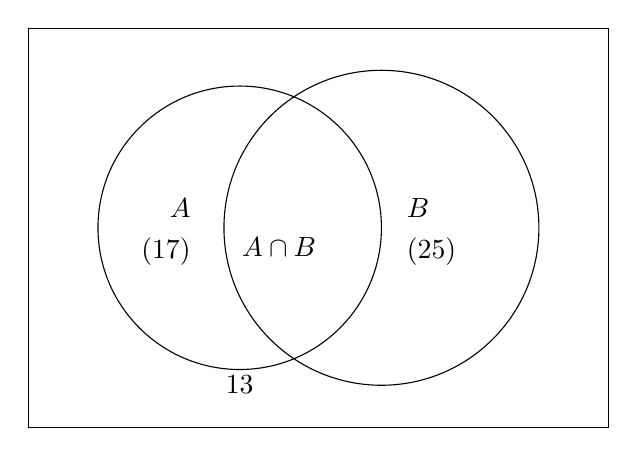
\begin{tikzpicture}[scale=1]
\def\radius{2cm}
\coordinate (ceni);
\coordinate[xshift=.9*\radius] (cenii);

\draw (ceni) circle (.9*\radius);
\draw (cenii) circle (\radius);
\draw  ([xshift=-25pt,yshift=15pt]current bounding box.north west)
rectangle ([xshift=25pt,yshift=-15]current bounding box.south east);

\path (-0.5,0) node[above left]{$A$};
\path (-0.5,0) node[below left]{$(17)$};
\path (2,0) node[above right]{$B$};
\path (2,0) node[below right]{$(25)$};
\path (0.5,0) node[below]{$A\cap B$};
\path (0,-1.75) node[below]{$13$};
\end{tikzpicture}}}
\end{ex}
\dongcham{18}
